\section{Abläufe}

Während in Kapitel 2 die Interaktion der Hauptkomponenten \textit{Server} und der \textit{RobotUnit} bzw. möglichen Kunden abgehandelt wurde, werden im Folgenden die Abläufe der innerhalb der Pakete genauer spezifiziert und auch interne Komponentenabläufe beschrieben.

\subsection*{Interaktion bei Ausführung von \textit{chooseRobot}}


\begin{figure}[H]
	\centering
	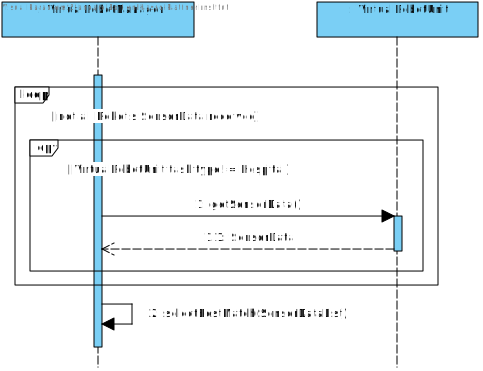
\includegraphics[width=0.85\textwidth]{img/8-chooseRobot}
	\caption{Sequenzdiagramm von \emph{chooseRobot}}
	\label{chooseRobotInteraktion}
\end{figure}
In der Hauptklasse \textit{VirtualRobotManager} der \textit{ServerSoftware} wird dieser Ablauf ausgeführt, wenn der zu einem zu verteilnden \textit{Task} am besten passendste \textit{VirtualRobotUnit} bzw. der dazugehörigen \textit{RobotUnit} ermittelt werden soll. Dabei werden Sensordaten von jeder \textit{RobotUnit}, der nicht gerade einen Krankenhaustransport ausführt, gesammelt. Diese werden anschließend in der Methode \texttt{selectBestMatch} ausgewertet.
\\

\subsection*{Interaktion bei Ausführung von \textit{readSensors}}


\begin{figure}[H]
	\centering
	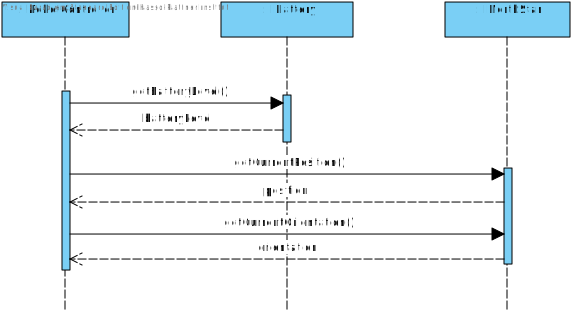
\includegraphics[width=1\textwidth]{img/8-readSensor}
	\caption{Sequenzdiagramm von \emph{readSensors}}
	\label{ReadSensorsInteraktion}
\end{figure}
Diese Interaktion ensteht innerhalb der \textit{RobotSoftware} in der Klasse \textit{RobotController} genau dann, wenn der \textit{Server} von allen \textit{RobotUnits} im Rahmen von \texttt{getSensorData} die Sensordaten von allen  \textit{RobotUnits} sammelt. Der \textit{RobotController} steuert dann die Hardware-Schnittstellen der \textit{RobotUnit} an und sammelt die Sensordaten.
\\
	
\subsection*{Interaktion bei Ausführung von \textit{driveToDestination}}


\begin{figure}[H]
	\centering
	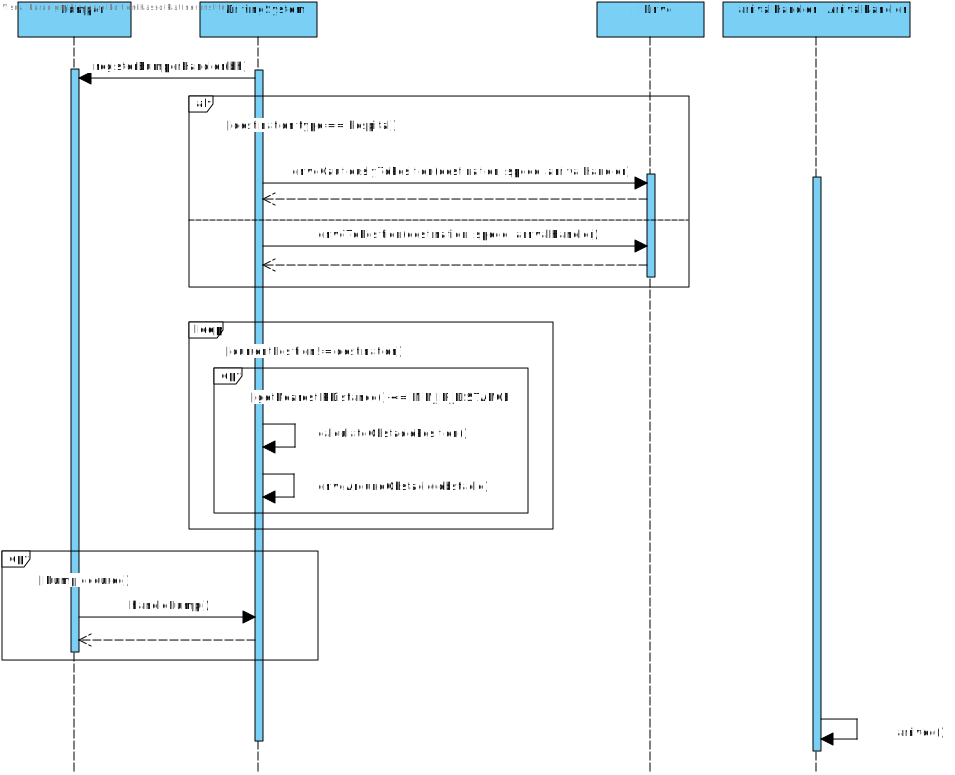
\includegraphics[width=1\textwidth]{img/8-DriveToDestination}
	\caption{Sequenzdiagramm von \emph{driveToDestination}}
	\label{driveToDestinationInteraktion}
\end{figure}
Diese Interaktion beschreibt das Verhalten der \textit{RobotSoftware} während der Anfahrt eines Ziels. Genauer wird die Interaktion zwischen der in der \textit{RobotUnit} für das fahren zuständige \textit{DrivingSystem} und den Hardwareschnittstellen die \textit{RobotUnit} modelliert. Der Vorgang wird duch einen möglichen Unfall unterbrochen. Zunächst überprüft das \textit{DrivingSystem}, ob es sich um einen Taxi- oder Hospitalauftrag handelt. Anhand dessen wird die Geschwindigkeit ermittelt, mit der die \textit{Destination} angefahren wird. Daraufhin wird mittels der Methode \textit{driveToPosition} das Ziel mit der festgelegten Geschwindigkeit angefahren. Nun kann es passieren, dass ein \textit{Obstacle} umfahren werden muss. Dieser Fall tritt auf, wenn das Interface \textit{IRDistance} einen zu geringen Abstand zu einem \textit{Obstacle} meldet. Ist dies der Fall, wird das \textit{Obstacle} mittels der Methode \textit{driveAroundObstacle} umfahren. Diese Überprüfungen finden solange statt, bis die \textit{Destination} erreicht wurde. Des Weiteren dient der \textit{IBumper} zur Lösung eines \textit{Bumps} mittels der Methode \textit{handleBump}.
\\

	
\subsection*{Interaktion bei Ausführung von \textit{requestRepair}}

\begin{figure}[H]
	\centering
	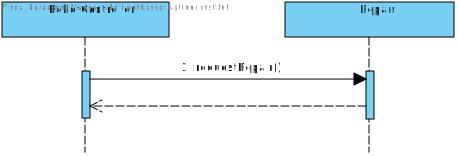
\includegraphics[width=0.81\textwidth]{img/8-requestRepair}
	\caption{Sequenzdiagramm von \emph{requestRepair}}
	\label{requestRepairInteraktion}
\end{figure}

Diese Interaktion entsteht dann, wenn ein \textit{RobotUnit} verunglückt. Dabei wird durch den \textit{BumperHandler} ausgelöst, dass in der Hauptklasse \textit{RobotController} der \textit{RobotSoftware} über die von uns definierte Schnittstelle \textit{IRepair} der \textit{Server} über den Unfall benachrichtigt wird.\\

\subsection*{Interaktion bei Ausführung von \textit{charging}}

\begin{figure}[H]
	\centering
	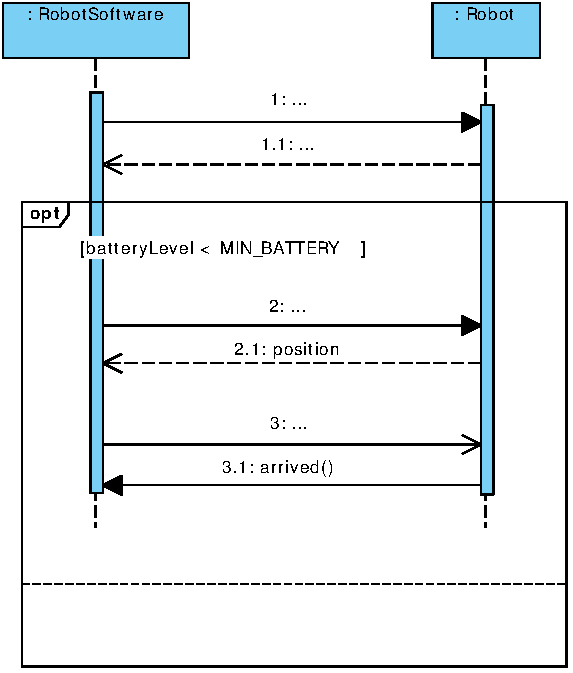
\includegraphics[width=1\textwidth]{img/0-Entwurf-8-Charging}
	\caption{Sequenzdiagramm von \emph{charging}}
	\label{chargingInteraktion}
\end{figure}

Diese Interaktion entsteht dann, wenn ein \textit{RobotUnit} gerade keinen \textit{Task} zum ausführen hat. Die \textit{RobotUnit} prüft dann, ob der aktuelle Akkustand unter einem vorher festgelegten Schwellwert liegt. Wenn dies der Fall ist, wird die Position der zugehörigen Ladestation von den Hardwareschnittstellen abgefragt und die \textit{RobotUnit} fährt die Ladestation an. \\
